\documentclass[../main.tex]{subfiles}
\begin{document}

\section{Билет 8. Теорема о единственности классического решения задачи Коши для волнового уравнения (на примере случая $\mathbb{R}^2$ ). Метод интеграла энергии.}


\begin{theorem} Классическое решение ЗК для волнового уравнения в $\mathbb{R}^n$ единственно.
\end{theorem}
\begin{proof}[Доказательство (для случая $\mathbb{R}^2$)]
Пусть $u_{1}$ и $u_{2}$ - классические решения.

Тогда функция $v(t,x) = u_{1}(t,x) - u_{2}(t,x)$ удовлетворяет полностью однородной задаче: 
\begin{equation*}
    \left\{
        \begin{matrix}
        v_{tt} - a^2(v_{x_1x_1} + v_{x_2x_2}) = 0\\
        v|_{t=0} = v_{t}|_{t=0} = 0
        \end{matrix}
    \right.
\end{equation*}
Наша цель - показать, что $v\equiv 0 $ в $ (t\geq 0, x\in \mathbb{R}^2) $.

Возьмем точку $ (t^0,x^0),\; t^0> 0,\; x^0\in\mathbb{R}^2 $. \; Выпустим из этой точки характеристическую поверхность - конус 
$$ 
w(t,x) = a^2(t - t^0)^2 - (x_1 - x_1^0)^2 - (x_2 - x_2^0)^2 = 0,\; t<t^0.
$$

Возьмем его часть - усечённый конус $ V_T $ с нижним основанием $ \Sigma_0 $, верхним $ \Sigma_T $  и боковой поверхностью $ \Gamma_T. $
\begin{center}
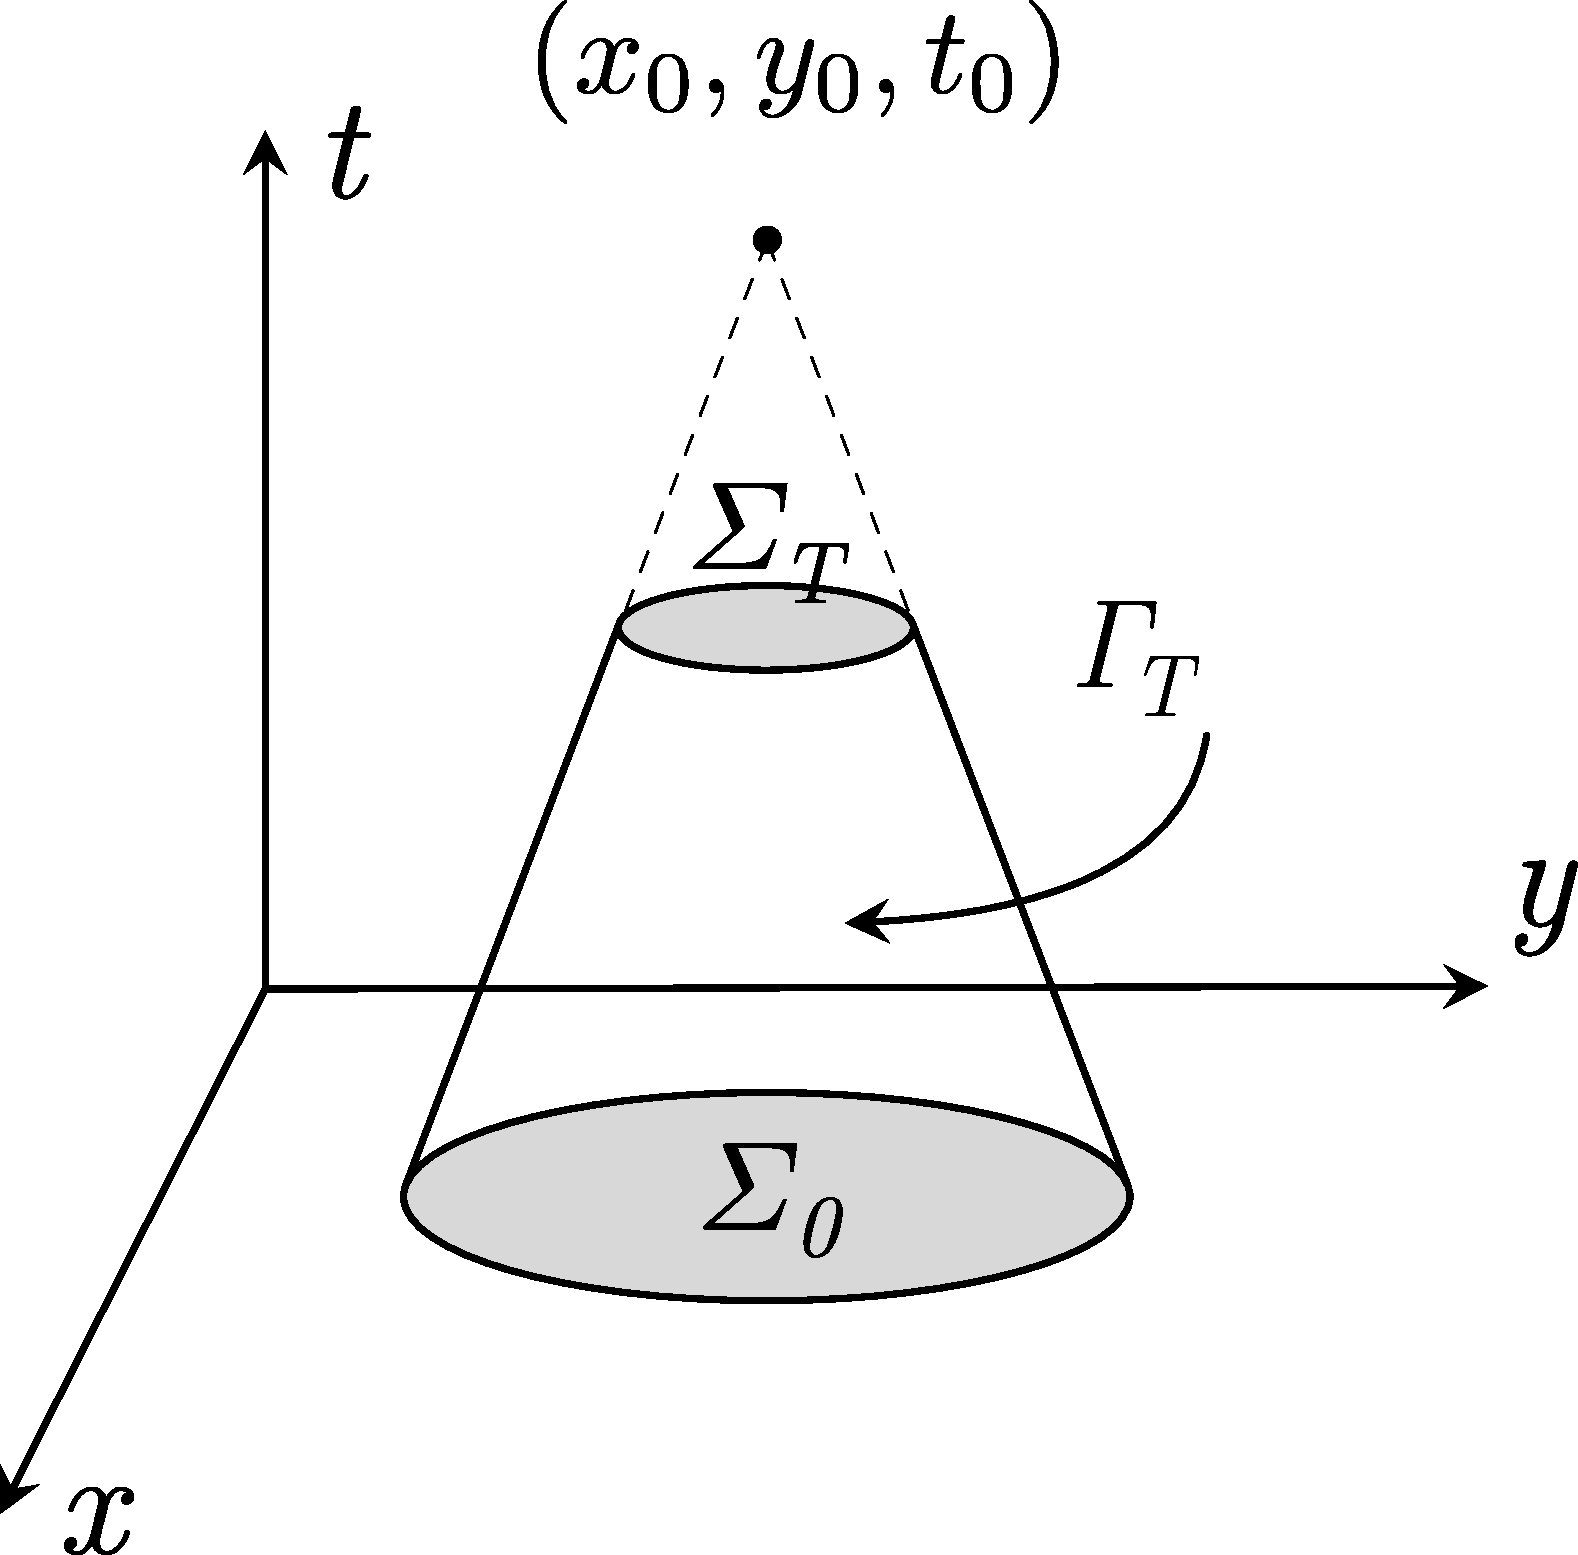
\includegraphics[width=0.28\linewidth]{pic 8.pdf}
\end{center}
Вектор (внешней) нормали $ \overrightarrow{n} $ к этому усеченному конусу:
\begin{itemize}
	\item на $\Sigma_T: \overrightarrow{n} = \begin{pmatrix}1 & 0 & 0\end{pmatrix}^T $
	\item на $\Sigma_0: \overrightarrow{n} = \begin{pmatrix}-1 & 0 & 0\end{pmatrix}^T $
	\item на $\Gamma_T:\overrightarrow{n}=\dfrac{-1}{\sqrt{w_t^2+w^2_{x_1}+w^2_{x_2}}}\begin{pmatrix}w_t\\w_{x_1}\\w_{x_2}\end{pmatrix}$. \; В силу соотношений $\; w_t^2 - a^2w^2_{x_1} - a^2w^2_{x_2} = 0 $ , имеем $n^2_t = a^2(n^2_{x_1} + n^2_{x_2})$.

Т.к. $n^2_t + n^2_{x_1} + n^2_{x_2} =1,\; n^2_t = \dfrac{a^2}{a^2 +1} \;\Rightarrow n_t = \dfrac{a}{\sqrt{a^2+1}}.$
\end{itemize}


Функция 
$ \;
\psi \equiv 0 = v_t(v_{tt}- a^2v_{x_{1}x_{1}} - a^2v_{x_{2}x_{2}})\equiv 0, \quad\text{во всех точках усеченного конуса.}
$ 

Раскроем скобки:
\begin{multline*}
    v_{t}v_{tt}-a^2v_{t}v_{x_1x_1}-a^2v_{t}v_{x_2x_2}= {} \\ {}=\frac{1}{2}(v^2_t)_t+a^2v_{x_1}v_{x_1t}-(a^2v_{t}v_{x_1})_{x_1}+a^2v_{x_2}v_{x_2t}-(a^2v_{t}v_{x_2})_{x_2}= {}\\ 
    {}=\frac{1}{2}(v^2_t)_t-(av_{t}v_{x_1})_{x_1}-(av_{t}v_{x_2})_{x_2}+\left(\frac{1}{2}a^2v^2_{x_1}\right)_t+\left(\frac{1}{2}a^2v^2_{x_2}\right)_t= {}\\ 
    {}=\brs{\frac{v^2_t+a^2v^2_{x_1}+a^2v^2_{x_2}}{2}}_t+(-a^2v_{t}v_{x_1})_{x_1}+(-a^2v_{t}v_{x_2})_{x_2} = {}\\
    {}=F^t_t + F^{x_1}_{x_1}+F^{x_2}_{x_2} \quad \text{---} \quad\text{дивергентный вид.}
\end{multline*}


Введем в рассмотрение векторное поле $ \overrightarrow{F} = \begin{pmatrix}F^t &F^{x_1}  &F^{x_2} \end{pmatrix}^T $. Тогда то выражение, к которому мы пришли, есть
$$
 \mathrm{div}\overrightarrow{F} = \frac{\partial }{\partial t}F^t + \frac{\partial }{\partial x_1}F^{x_1} + \frac{\partial }{\partial x_2}F^{x_2}.
$$

Проинтегрируем эту дивергенцию по объему усеченного конуса:
\begin{multline*}
  0=\iiint\limits_{V_T}\mathrm{div}\overrightarrow{F} = \oiint\limits_{\partial V_T}(\overrightarrow{F},\overrightarrow{n})\mathrm{d}S = {}\\
  {} =\iint\limits_{\Sigma_T}\frac{v^2_t+a^2v^2_{x_1}+a^2v^2_{x_2}}{2}\mathrm{d}S-\iint\limits_{\Sigma_0}\frac{v^2_t+a^2v^2_{x_1}+a^2v^2_{x_2}}{2}\mathrm{d}S + {}\\
  {} +\frac{1}{2}\iint\limits_{\Gamma_T}\brs{(v^2_t+a^2v^2_{x_1}+a^2v^2_{x_2})n_t-2a^2v_{t}v_{x_1}n_{x_1} - 2a^2v_{t}v_{x_2}n_{x_2}}\mathrm{d}S = {}\\
  {} = E(\Sigma_T) + E(\Gamma_T) - E(\Sigma_0) 
\end{multline*}

В силу начальных условий $ v|_{t=0}=0 $ и $ v_t|_{t=0} $, имеем $ E(\Sigma_0)=0 $ (под интегралом тождественный ноль).

Тогда $ E(\Sigma_T)+E(\Gamma_T)=0 $. 
Кроме того, $ E(\Sigma_T)\geq 0 $ (под интегралом сумма квадратов).

Покажем, что и $ E(\Gamma_T)\geq 0 $: разделим и домножим её на $ n_t=\dfrac{a}{\sqrt{a^2+1}} $

\begin{multline*}
  \frac{1}{2}\frac{\sqrt{a^2+1}}{a}\iint\limits_{\Gamma_T}\brs{(v^2_t+a^2v^2_{x_1}+a^2v^2_{x_2})n^2_t \; - \; 2a^2v_{t}v_{x_1}n_tn_{x_1} \; - \; 2a^2v_{t}v_{x_2}n_tn_{x_2}}\mathrm{d}S = {}\\
  {} =\frac{1}{2}\frac{\sqrt{a^2+1}}{a}\iint\limits_{\Gamma_T}\brs{v^2_ta^2(n^2_{x_1} + n^2_{x_2})\; + \; a^2v^2_{x_1}n^2_t \; + \; a^2v^2_{x_2}n^2_t\; - \; 2a^2v_{t}v_{x_1}n_tn_{x_1} \; - \; 2a^2v_{t}v_{x_2}n_tn_{x_2}}\mathrm{d}S = {}\\
  {} = \frac{1}{2}a\sqrt{a^2+1}\iint\limits_{\Gamma_T}\brs{(v_tn_{x_1} -v_{x_1}n_t)^2+(v_tn_{x_2}-v_{x_2}n_t)^2}\mathrm{d}S\geq 0  
\end{multline*}

Значит, $ E(\Sigma_0)=E(\Sigma_T)=E(\Gamma_T)\equiv 0.$
\; Из $ E(\Sigma_T)\equiv0 $ получаем: 
$$ v_t\equiv0; v_{x_1}\equiv0; v_{x_2}\equiv0 \; \Rightarrow \triangledown v  = 0 \; \Rightarrow v = const = v|_{t=0}=0 
$$
Это верно всюду внутри усеченного конуса.
Заметая такими конусами всё пространство, получим, что $ v \equiv 0 $.
\end{proof}
\end{document}